\chapter{Resultat}
\label{cha:results}
I detta kapitel presenteras resultaten som projektet har genererat. Resultaten är bland annat den faktiska webbapplikation som producerats samt de erfarenheter som gruppen dragit på sig under projektets gång. Det ges även en kort översikt av de individuella fördjupningar som gruppens medlemmar genomfört.
\section{Testning}
Under projektets gång utvecklade gruppen en testmetodik för att kunna verifiera att applikationen möter de krav som etablerats i kravspecifikationen. Vid projektets start skapades en övergripande testplan som beskrev en förlaga till den testmetodik som utvecklades under projektet. Då gruppen såg framtagandet av testningsprocesser som ett kontinuerligt arbete så kunde dessa utvecklas inkrementellt utifrån gruppens erfarenheter, färdigheter och förväntningar från tidigare iterationer. Vartefter projektet fortlöpte tillkom testuppgifter, olika testverktyg utvärderades och metoder för att frambringa spårbarhet i testningsprocessen togs fram. Detta resulterade i ett ramverk för testning anpassat för mindre utvecklingsgrupper arbetandes efter agila principer.

\section{Prototyper}
\label{sec:result-prototypes}
De slutgiltiga övergripande prototyperna skapades i pappersform, och gjordes delvis interaktiva i verktyget InVision. 

\begin{figure}[H]
    \centering
    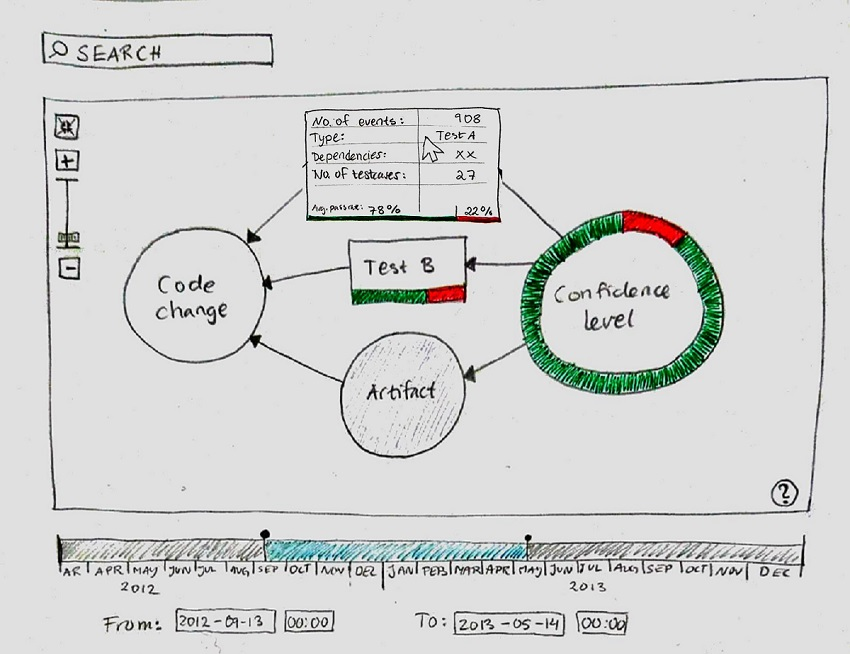
\includegraphics[scale=0.65]{prototype-aggregation}
    \caption{Prototyp för den aggregerade vyn och händelse vid placering av muspekaren på en nod.}
    \label{fig:prototype-aggregation}
\end{figure}
\ \\
Skiss för den aggregerade vyn syns i figur \ref{fig:prototype-aggregation}. 
I skissen finns en yta för en aggregerad graf, där grafens noder representerar en händelsetyp i KI-flödet. 
De flerfärgade noderna illustrerar grad av godkända körningar för den händelsetypen. Den översta noden i mitten visar en förstorad nod då muspekaren placeras på noden. 
Rutan innehåller mer detaljerad information om händelserna i noden. Vid klick på rutan navigerar applikationen till nästa vy. 
Grafens ruta inkluderar även en navigeringspanel med zoom-reglage, samt en ikon för hjälp. 
Under grafens ruta finns en tidslinje för att filtrera ut händelser från ett visst tidsspann. 

\begin{figure}[H]
    \centering
    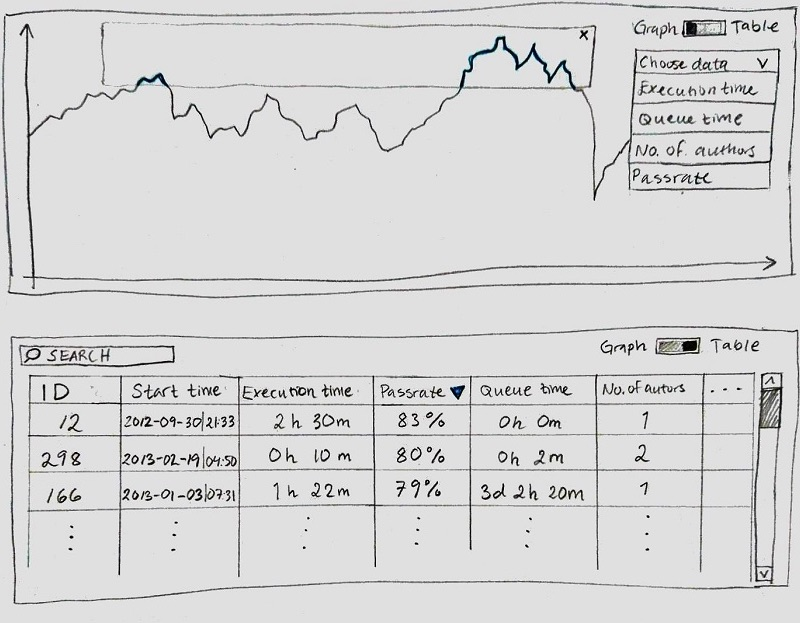
\includegraphics[scale=0.5]{niva2}
    \caption{Prototyp för diagramläget samt tabelläget för den detaljerade vyn.}
    \label{fig:prototype-details}
\end{figure}
\ \\
I figur \ref{fig:prototype-details} visas prototypen för den detaljerade vyn, som innehåller detaljer om en specifik händelsetyp. 
Där kan användaren välja att visa ett tabelläge eller ett diagramläge. Tabelläget visar en rad för varje händelse i noden, och den kan sorteras baserat på alla kolumner. 
Vid växling till diagramläget visas olika data för noden över tid. 
På den horisontella axeln visas tid, och på den vertikala axeln kan användaren välja någon data genom att bläddra i rullistan. 

\begin{figure}[H]
    \centering
    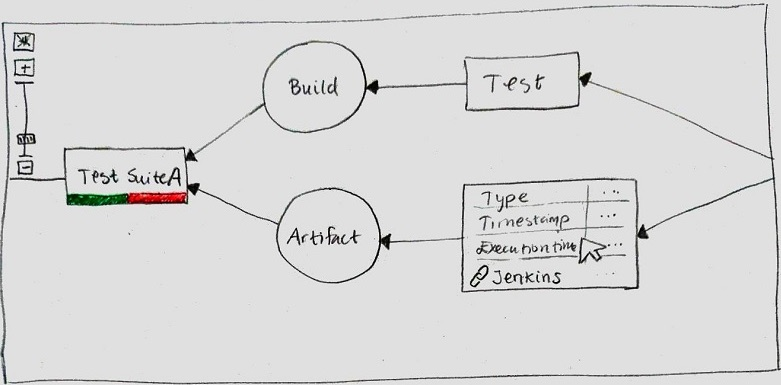
\includegraphics[scale=0.5]{niva3}
    \caption{Prototyp för ett händelseflöde.}
    \label{fig:prototype-eventchain}
\end{figure}
\ \\
Den tredje vyn är en graf som visar ett enskilt händelseflöde, se figur \ref{fig:prototype-eventchain}. 
I denna graf är varje nod en specifik händelse. 
I den förstorade rutan vid placering av muspekare på en nod finns en länk för att öppna händelsen i programmet som genererade den.

\section{Systembeskrivning}
Denna del beskriver det system som gruppen har tagit fram och ger en överblick på hur systemet fungerar.
\label{sec:results-systemoverview}
\begin{figure}[h]
    \centering
    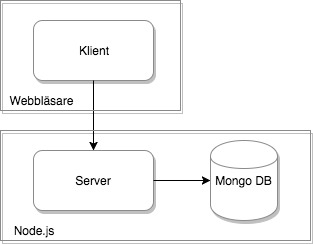
\includegraphics[scale=0.5]{Systemskiss}
    \caption{Översikt av systemet.}
    \label{fig:architectural_overview}
\end{figure}
\\
En översikt av systemet ges i figur.\ref{fig:architectural_overview} Systemet består av en klient och en server. Både klienten och servern har utvecklats i ramverket Meteor för JavaScript. Servern sköter all hämtning av data från databasen och levererar den till klienten. Klienten används för all visualisering av Eiffeldata. Den hämtar Eiffelhändelser från servern och visualiserar dom i webbläsaren. De Eiffelhändelserna sparas ner i en lokal databas med namnet Mini Mongo. Klienten är en \textit{Single-page application} vilket betyder att sidan bara behöver laddas en gång när den startas, så att de individuella delarna på sidan uppdateras dynamiskt utan att behöva ladda om sidan som leder till en bättre användarupplevelse.
\\ \\
Applikationens filstruktur följer Meteors rekommenderade standard.\cite{website:meteorstructure} Den följer även Meteors rekommenderade kodstil för hur kod till en applikation implementeras.\cite{website:meteorcodestyle} En tydlig struktur för projektet ger applikationen en enhetlig standard vilket ökar läsbarheten för utvecklaren.

\subsection{Systemanatomi}
\label{subsec:results_anatomy}
En systemanatomin togs fram baserat på de funktionella kraven från kravspecifikationen och användningsfall.
\begin{figure}[H]
    \centering
    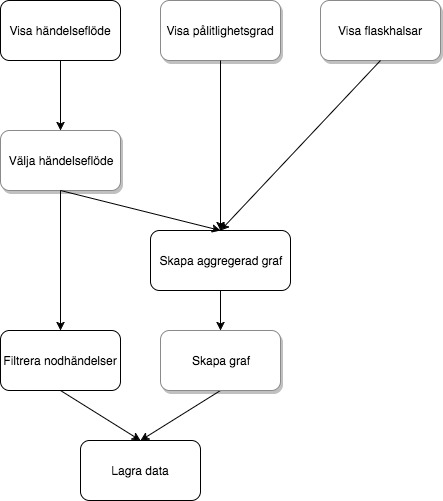
\includegraphics[scale=0.35]{Systemanatomi}
    \caption{Systemets anatomi.}
    \label{fig:systemanatomi}
\end{figure}
\ \\I figur \ref{fig:systemanatomi} visas systemanatomin för applikationen. Där de primära användarfunktioner för systemanatomin är högst upp i figuren.

\subsection{Moduler}
\label{subsec:results-modules}
\begin{figure}[h]
    \centering
    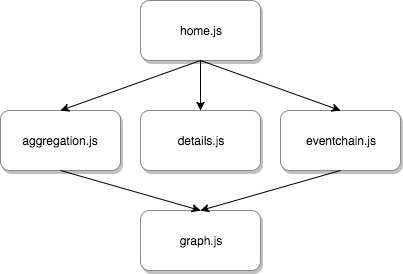
\includegraphics[scale=0.5]{moduler}
    \caption{Översikt av klientens moduler.}
    \label{fig:module_overview}
\end{figure}
\ \\
I figur \ref{fig:module_overview} ges en översikt över de moduler som används i applikationen. Applikationens klient är uppdelad i fyra moduler som hanterar de olika typer av funktionalitet som används. I följande lista finns de modulerna och deras uppgift.
\begin{itemize}
  \item Aggregation.js - Innehåller de funktionsanrop som behövs i de aggregerade graferna.
  \item Eventchain.js - Innehåller de funktionsanrop som behövs när en nod från den aggregerade grafen visas i tabelläge eller diagramläge.
  \item Details.js - Innehåller funktionsanrop för händelseflöde och har precis som aggregation.js i uppgift att rendera grafer.
  \item Graph.js - Är modulen där all rendering av grafer för aggregering och händelseflöden sker. Graph.js använder sig av två externa bibliotek: Cytoscape.js för rendering av graferna och Dagre.js för dess layout.
\end{itemize}

\section{Användargränssnitt}
\label{sec:results-gui}
%\textbf{TODO:}
%\begin{itemize}
%\item Ändra färgers representation om dessa ändras i GUI:t
%\item Hjälprutans innehåll
%\end{itemize}
Systemet visar data i tre olika vyer. De tre vyerna är placerade under varandra och vid start presenteras den översta vyn. För att navigera mellan de olika vyerna finns dels funktionalitet i varje vy som beskrivs i följande avsnitt, men också en allmän navigationspanel på höger sida. Vid klick på knapparna för vyerna kommer det visade området att förflyttas till den valda vyn. Hela panelen följer med och syns alltid på skärmen oavsett vilken vy som visas.

\begin{figure}[H]
  \centering
  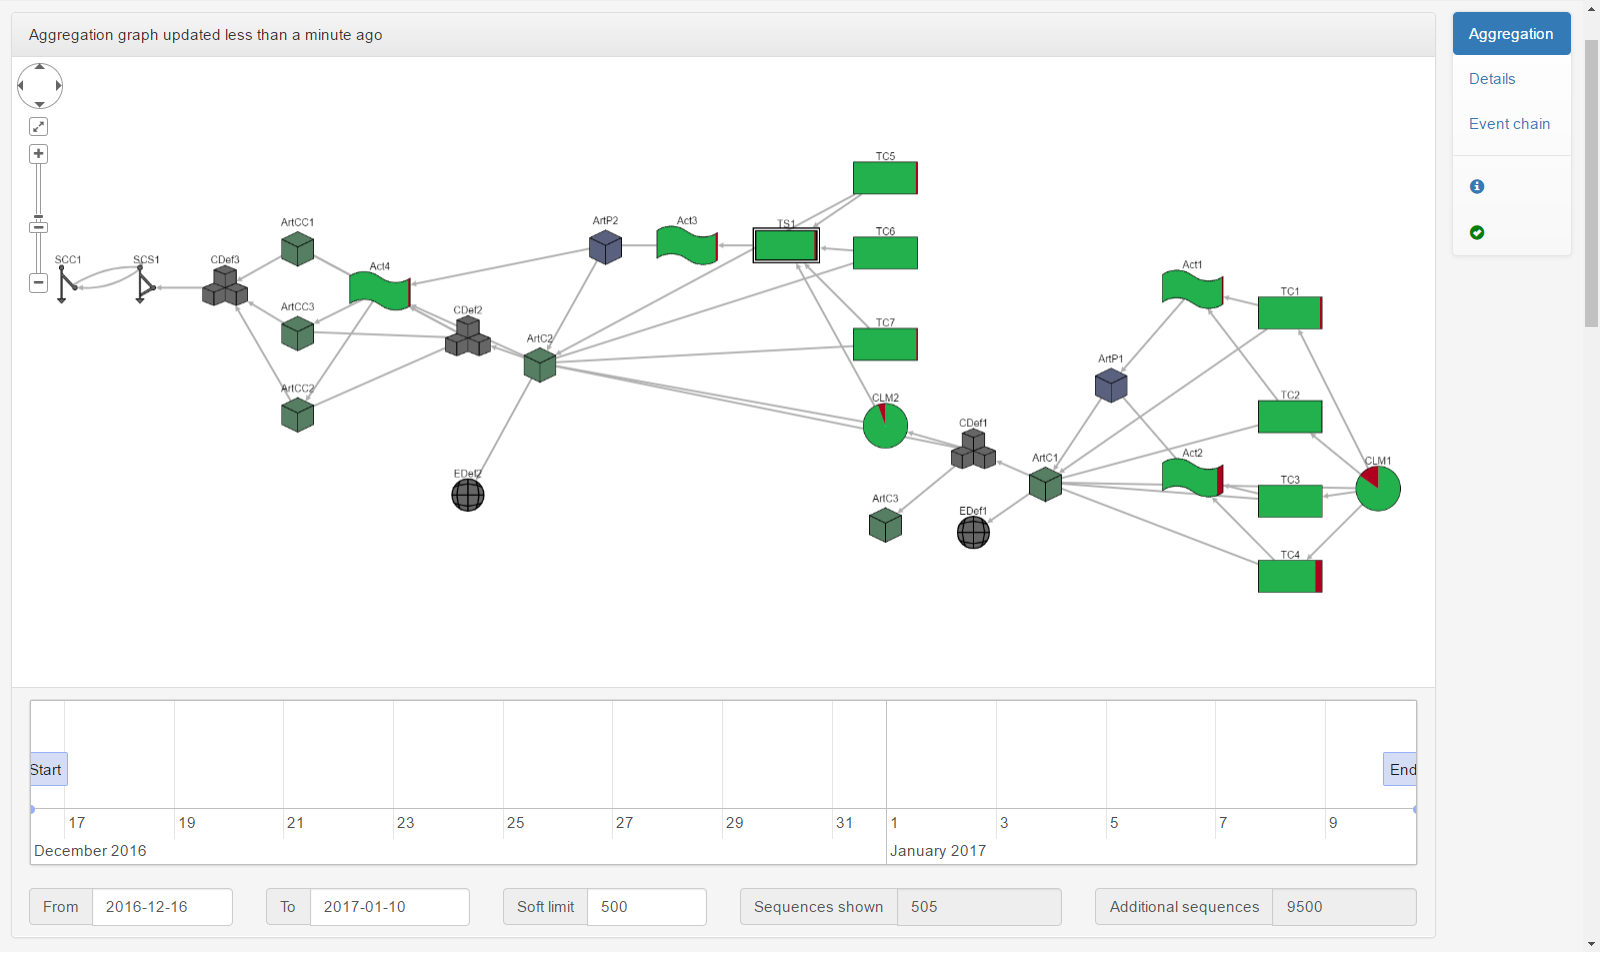
\includegraphics[scale=0.33]{gui_aggregation}
  \caption{Aggregeringsvyn med navigationspanelen till höger.}
  \label{fig:gui_aggregation}
\end{figure}
\ \\
Panelen innehåller även informationsknapp för att öppna en hjälpruta, samt en indikator för uppkoppling mot servern, vilket visas till höger i figur \ref{fig:gui_aggregation}.  

\begin{figure}[H]
  \centering
  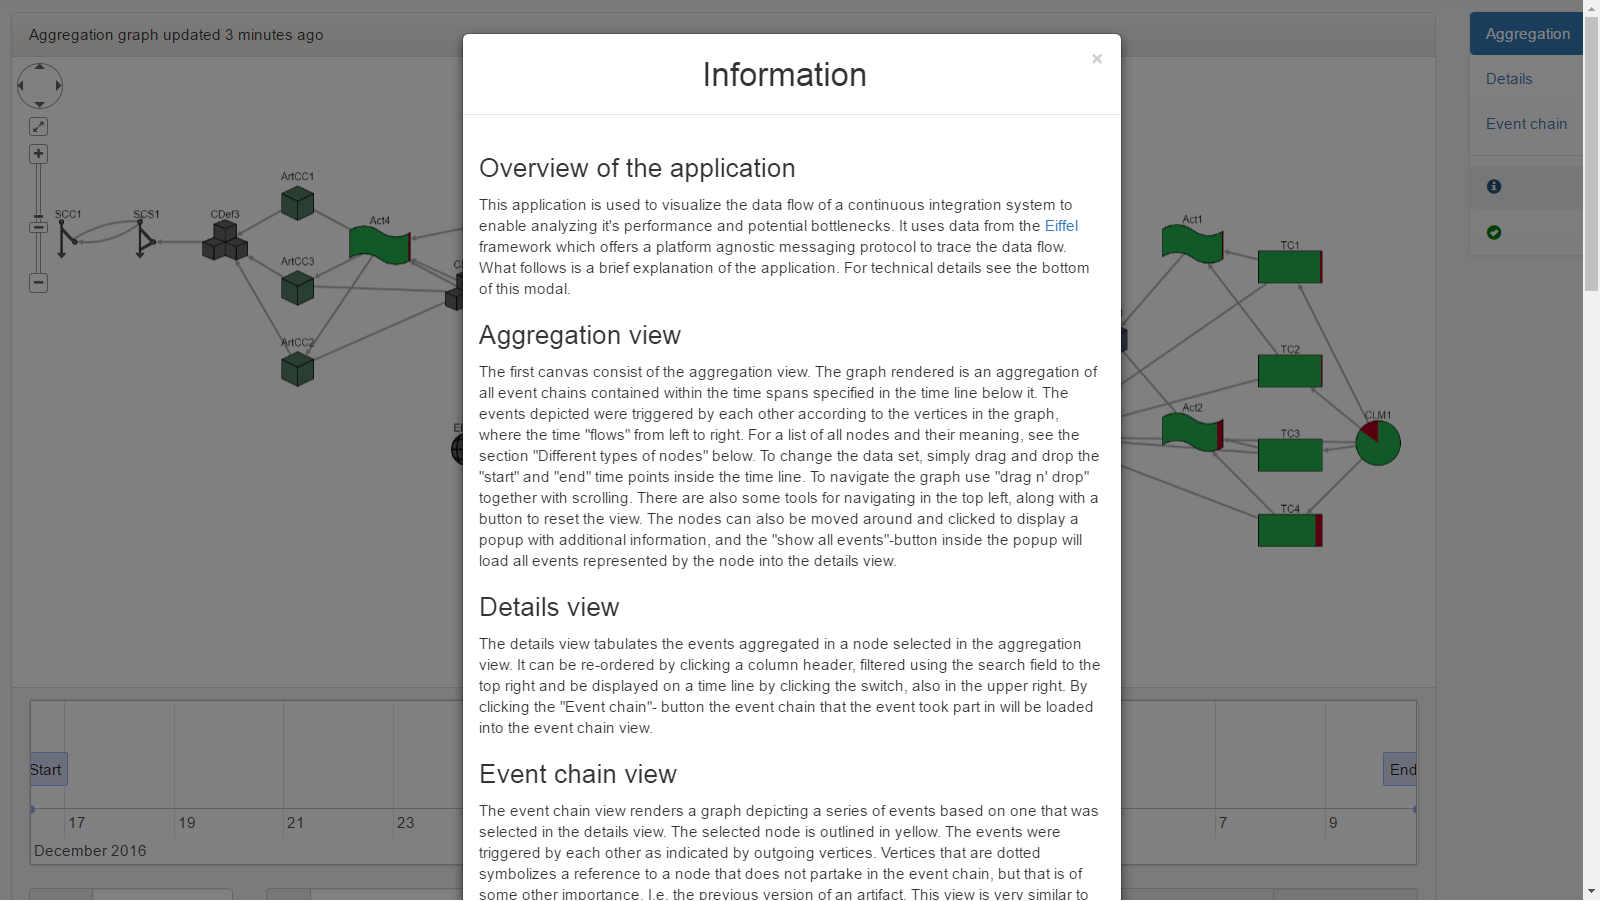
\includegraphics[scale=0.33]{gui_helpmodal}
  \caption{Hjälprutan har öppnats ovanpå den aggregerade vyn.}
  \label{fig:gui_helpmodal}
\end{figure}
\ \\
Hjälprutan som visas i figur \ref{fig:gui_helpmodal} innehåller information om hur applikationen används.

\begin{figure}[H]
  \centering
  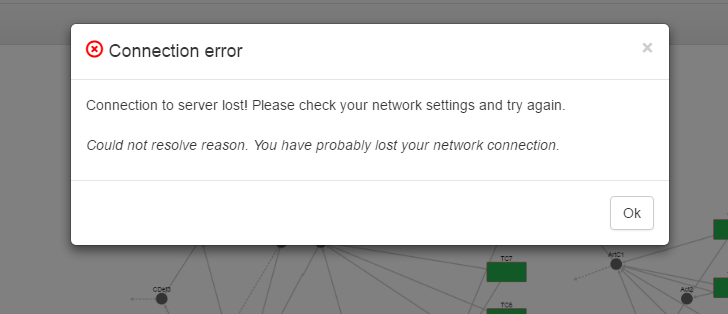
\includegraphics[scale=0.6]{gui_connection}
  \caption{Informationsruta som dyker upp om klienten tappar kontakten med servern.}
  \label{fig:gui_connection}
\end{figure}
\ \\
Indikatorn för uppkoppling mot server är grön då klienten är ansluten till servern. Vid tappad anslutning dyker en informationsruta upp som informerar om att anslutningen är bruten samt eventuell anledning, se figur \ref{fig:gui_connection}. Indikatorn blir då röd.

\begin{figure}[H]
  \centering
  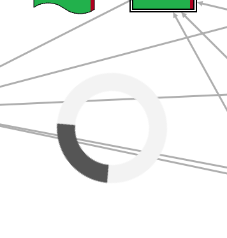
\includegraphics[scale=0.8]{gui_loading}
  \caption{Symbol för att indikera att klienten väntar på svar från servern.}
  \label{fig:gui_loading}
\end{figure}
\ \\
I figur \ref{fig:gui_loading} syns symbolen som roterar över skärmen då klienten väntar på svar på ett anrop till servern.

\subsection{Aggregering}
Aggregeringen representeras av en riktad acyklisk graf, och visar Eiffel-händelser som skett i KI-flödet, se figur \ref{fig:gui_aggregation}. Varje nod i grafen är en typ av händelse, och innehåller i sin tur varje enskild händelse av den typen. Bågarna pekar på den föregående händelsen i flödet. Noderna har olika former baserat på dess händelsetyp.
\\ \\
Vissa noder är händelser som har en status, exempelvis av implementationen definierade aktiviteter, eller körningar av testfall och testsviter. Dessa noder har olika färgfyllningar beroende på dess status. En nod för testfall som har 70\% klarade fall kommer att visas som en ruta med 7/10 grönt och 3/10 rött. 

\begin{figure}[H]
  \centering
  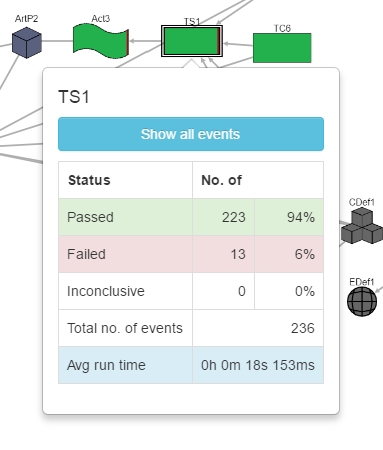
\includegraphics[scale=0.8]{gui_aggregation_tooltip}
  \caption{En informationsruta öppnas vid klick på en nod.}
  \label{fig:gui_aggregation_tooltip}
\end{figure}
\ \\
Vid klick på en nod dyker en informationsruta upp, som är kopplad till noden, se figur \ref{fig:gui_aggregation_tooltip}. Rutan innehåller mer detaljerad information, som till exempel antal händelser i noden och mer detaljer om händelsernas eventuella status. Informationsrutan innehåller även en knapp för att öppna den detaljerade vyn för den valda händelsetypen.
\\ \\
Under grafen visas en tidslinje, där det är möjligt att filtrera vilka händelser som visas, se figur \ref{fig:gui_aggregation}. Användaren kan zooma in i tidslinjen genom att scrolla, och då kommer varje steg i tidslinjen representeras av en mindre enhet tid. Minsta möjliga enhet är 10 minuter. 
Det finns två flyttbara markörer, en för starttid och en för sluttid. Vid förflyttning av dessa skickas ett anrop till servern som returnerar en ny filtrering av händelser. Markörerna kan maximalt flyttas till de tidpunkter då den första respektive sista händelsen i databasen ägde rum. Användaren kan även välja start och sluttid genom att fylla i boxarna för start och sluttid under tidslinjen.

\subsection{Detaljerad vy över en händelsetyp}
Den detaljerade vyn visar all data för varje händelse. Denna vy har två olika lägen, ett tabelläge och ett diagramläge. 
\begin{figure}[H]
  \centering
  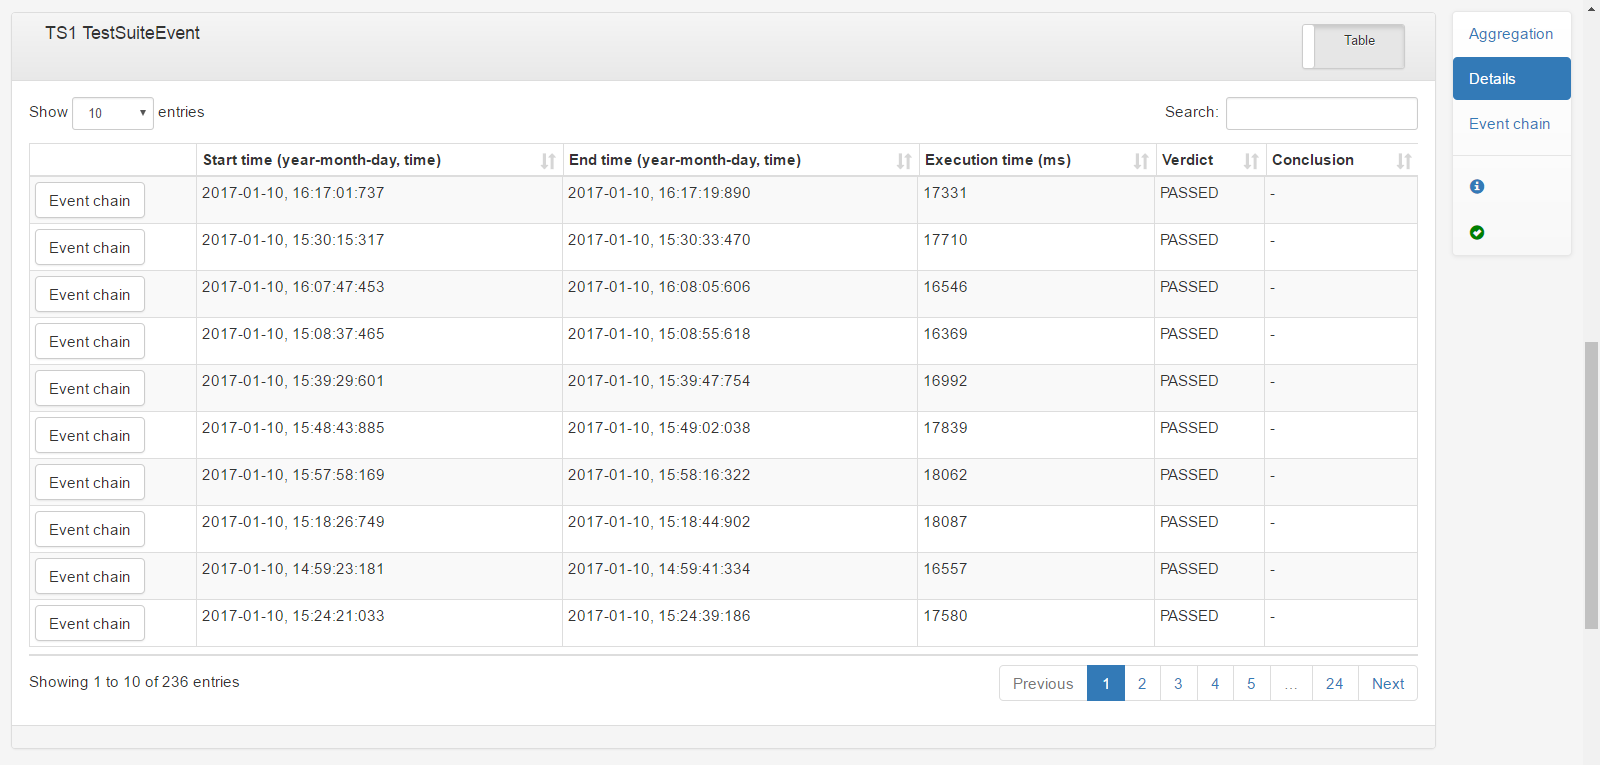
\includegraphics[scale=0.33]{gui_details}
  \caption{Den detaljerade vyns tabelläge.}
  \label{fig:gui_details}
\end{figure}
\ \\
I tabelläget som öppnas som standard visas varje enskild händelse som en rad i tabellen, se figur \ref{fig:gui_details}. Tabellen har kolumner som speglar varje händelsetyps datainnehåll, till exempel tidsstämpel eller teststatus. Det är möjligt att sortera tabellen i stigande eller fallande ordning med avseende på valfri data genom att klicka på kolumnens rubrik. Då dyker en symbol upp som visar i vilken ordning det är sorterat. Varje rad innehåller en knapp för att navigera till händelseflödet för den aktuella händelsen.
\begin{figure}[H]
  \centering
  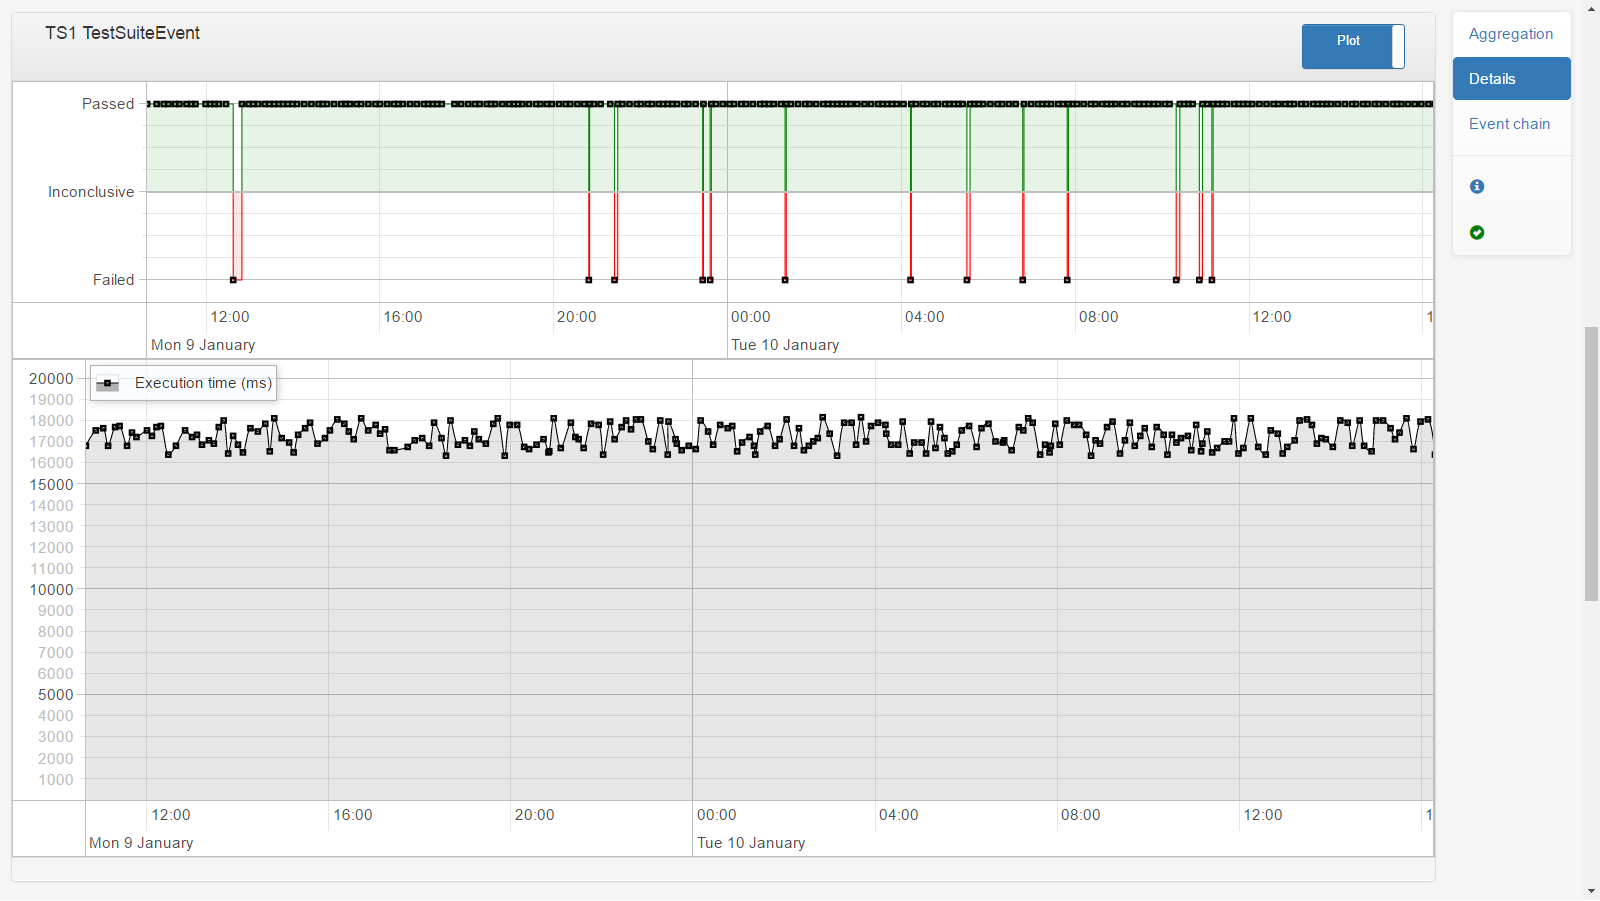
\includegraphics[scale=0.33]{gui_details_plot}
  \caption{Den detaljerade vyns diagramläge.}
  \label{fig:gui_details_plot}
\end{figure}
\ \\
Reglaget ovanför tabellen används för att navigera till diagramläget, se figur \ref{fig:gui_details_plot}. I diagramläget visas en funktionskurva som visar förändringar över tid hos en viss data i händelsetypen.

\subsection{Händelseflöden}
Ett händelseflöde representeras av en liknande graf som i aggregeringen. Skillnaden är att denna vy inte är aggregerad, alltså är varje nod en enskild händelse. 
\begin{figure}[H]
  \centering
  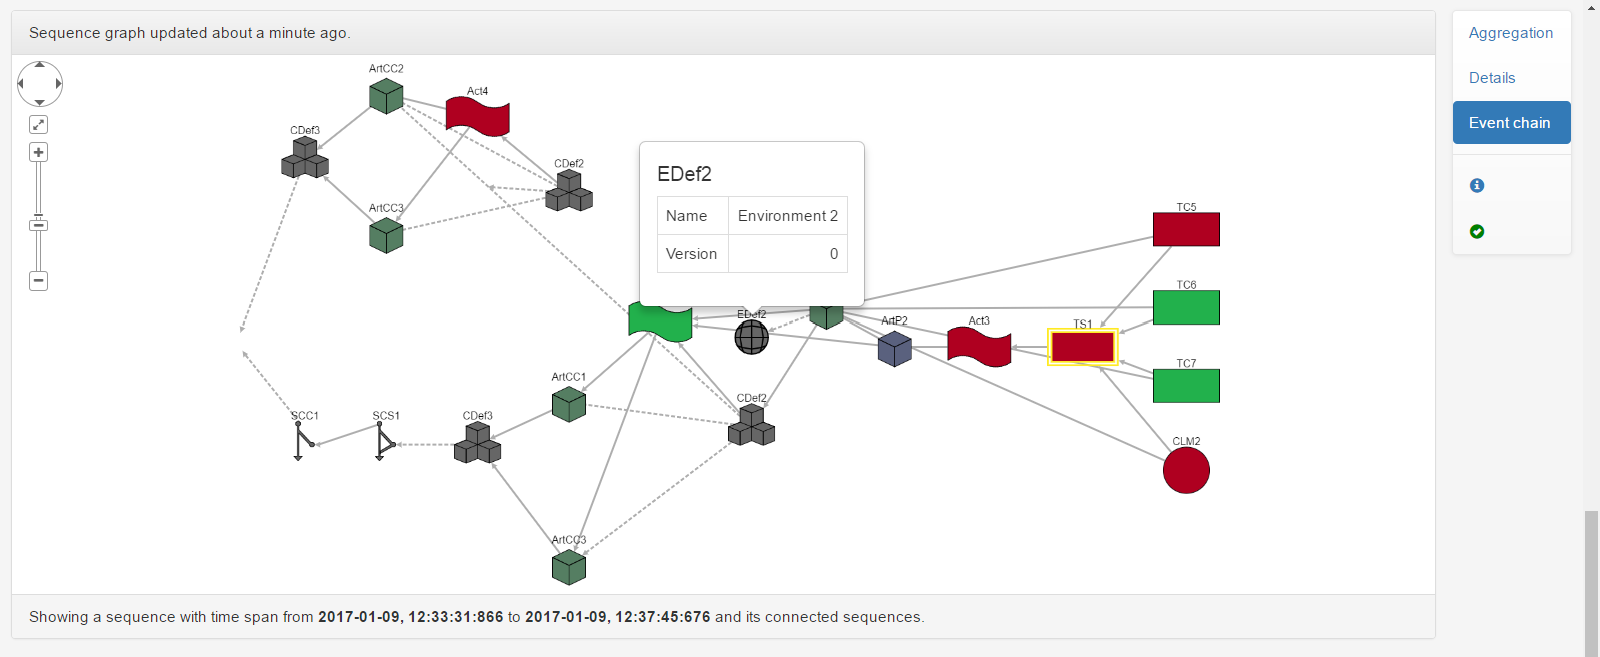
\includegraphics[scale=0.33]{gui_eventchain_tooltip}
  \caption{Ett händelseflöde, med en öppnad informationsruta.}
  \label{fig:gui_eventchain_tooltip}
\end{figure}
\ \\
Varje händelseflöde inleds med en kodändring, men då alla kodändringar är länkade till varandra i ett cykliskt beroende kapas länkarna från dessa och skapar \textit{sekvenser} av de resterande händelserna fram till en förändring av pålitlighetsgrad.
En händelse tillhör exakt en sekvens, men kan ha kopplingar till händelser i separata sekvenser. Detta kopplingar är oföljda länkar och representeras i grafen med streckade bågar. Den närmast närliggande sekvensen ritas ut, men dess egna oföljda länkar visas inte. På så sätt innehåller varje händelseflöde en eller flera sekvenser, med en kodändring som initiering.
\\ \\
Denna graf visar händelsetyp för varje nod samt eventuell status precis som i den aggregerade grafen, men då noderna endast representerar en händelse är de enfärgade. Den händelse som valdes i den detaljerade vyn framhävs i grafen genom att omges av en gul skugga. Även dessa noder är klickbara och visar då en informationsruta, vilket visas i figur \ref{fig:gui_eventchain_tooltip}. Rutan innehåller detaljerad data om händelsen, samt en länk till programmet som genererade händelsen. %, till exempel Jenkins.
\\ \\
En händelsetyp som hanteras annorlunda i händelseflöden är testsviter. Sviter innehåller körningar av flera testfall, och körningarna av dessa testfall visualiseras genom att dess händelser visas i den detaljerade vyn.

\section{Gemensamma erfarenheter}
\label{sec:results-experiences}
Nedan redogörs för vilka tidigare erfarenheter projekgruppen hade vid projektets start, samt hur gruppen utvecklades till projektets slut.

\subsection{Tidigare erfarenheter}
Den här sektionen presenterar de erfarenheter som projektgruppen hade när projektet började och de erfarenheter som medlemmarna fått under projekttidens gång.
Alla utom en av projektgruppens medlemmar hade genomfört ett projekt av liknande magnitud tidigare. Då detta projekt delar många aspekter med den tidigare projektkursen så kunde många av gruppens medlemmar känna en viss kunskap kring vad som förväntades av projektet. Den kunskap som kändes mest relevant var den kring hur mycket dokumentation som krävdes för den här typen av projekt. Att vissa medlemmar visste hur gruppen skulle komma igång med dokumentationen underlättade mycket då det var en del dokumentation i början av projektet.

\subsection{Nya erfarenheter}
De erfarenheter som gruppen har fått i och med detta projekt är främst erfarenheter relaterade till att jobba med andra människor i grupp och gruppdynamik. Andra erfarenheter som erhållits är sådana relaterade till webbprogrammering såsom inom HTML och JavaScript, samt dokumentationsrelaterade såsom LaTeX. Den erfarenhet som gruppen har uppskattat mest är den om hur man jobbar tillsammans i grupp då denna erfarenhet har gett mest värde inför framtida arbeten.


\section{Överblick över individuella undersökningar}
\label{sec:result-individual}
Denna del avser att presentera de individuella fördjupningsområden som gruppens medlemmar valt att fördjupa sig inom.

\begin{itemize}
\item \textit{Anpassning av testmetoder för småskalig utveckling} av Joakim Argillander
\item \textit{Kodgranskning som en kvalitetsmetod} av Victor Bodin
\item \textit{Användandet av workshops för kompetensutveckling} av Sebastian Callh
\item \textit{Prototypers påverkan på utveckling av användargränssnitt} av Rebecca Lindblom
\item \textit{Retrospective - Hur det hjälper team att effektivisera sitt arbete} av Johan Nåtoft
\item \textit{Utveckling med Meteor} av Johan Thornström
\item \textit{Hur vi använt de verktyg vi valt för utveckling av mjukvara} av Jonathan Wahlund
\item \textit{Val av verktyg vid projektdokumentation} av Daniel Wassing
\end{itemize}

%(RESULTAT
%I detta kapitel ska resultaten presenteras. Notera att resultaten
%ska presenteras rent faktamässigt, och så objektivt det bara
%går. De ska inte analyseras, diskuteras eller värderas. Detta
%lämnas till diskussionskapitlet.
%- 3 -
%Om metodkapitlet delats in i underrubriker såsom förstudie,
%design, implementation och utvärdering, ska resultatkapitlet
%också ha dessa underrubriker. Detta ger en tydligare röd tråd
%och gör kapitlet lättare att skriva.
%I de fall resultat redovisas från en process (till exempel en
%design- eller implementationsprocess), ska de viktigaste
%besluten som fattats under processens gång tydligt redovisas
%och motiveras. I normalfallet ska alternativa angreppssätt,
%etc, redan ha beskrivits i teorikapitlet, så det ska gå att
%hänvisa till detta kapitel som en del i motiveringen. Beslut
%och motiveringar identifieras i den processdokumentation
%(t.ex. idélogg, annoterad skissbok eller forskningsdagbok)
%som förts under genomförandet.)







%This chapter presents the results. Note that the results are presented
%factually, striving for objectivity as far as possible.  The results
%shall not be analyzed, discussed or evaluated.  This is left for the
%discussion chapter.

%In case the method chapter has been divided into subheadings such as
%pre-study, implementation and evaluation, the result chapter should
%have the same sub-headings. This gives a clear structure and makes the
%chapter easier to write.

%In case results are presented from a process (e.g. an implementation
%process), the main decisions made during the process must be clearly
%presented and justified. Normally, alternative attempts, etc, have
%already been described in the theory chapter, making it possible to
%refer to it as part of the justification.
